\chapter{MARCO PRACTICO}
\section{Análisis del Desempeño Económico}
La inversión pública es aquel gasto con fines productivos que realiza el Estado a través del gobierno central o de las autoridades subnacionales o locales. Este tipo de inversión se destina principalmente a proveer bienes, servicios o infraestructuras que sean consideradas básicas o importantes. Tenemos el caso, por ejemplo, de la seguridad ciudadana.

Cabe señalar que la inversión pública suele ser medida cada año, expresándose como un porcentaje del producto interior bruto (PIB). Entre los aspectos clave de la inversión pública destacan, se justifica en que hay bienes o servicios que un privado no puede proveer de forma eficiente, es decir, generando beneficios. Por lo tanto, ante la ausencia de oferta, el Estado debe intervenir 

\section{Análisis del PIB}
\begin{figure}[!h]
	\centering
%	\captionsetup{justification=centering}
\caption{\label{fig:Pib}Tasa de Crecimiento del Producto Interno Bruto\\ (En porcentaje)}
	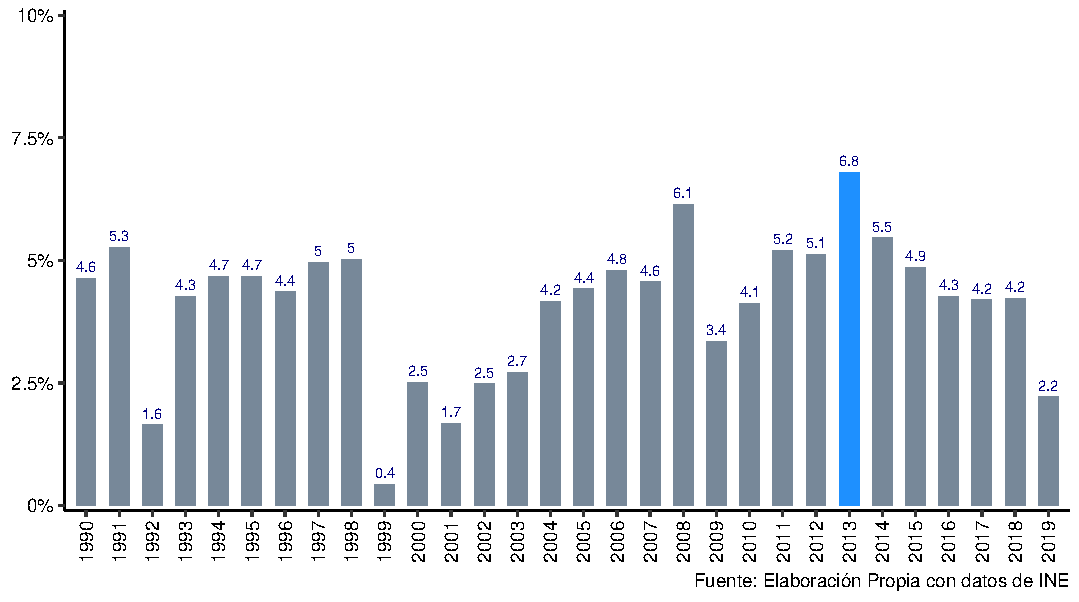
\includegraphics[scale=0.7]{Imagenes/pib_real_tasa.pdf}	
\end{figure}

Entre los aspectos clave de la inversión pública destacan, se justifica en que hay bienes o servicios que un privado no puede proveer de forma eficiente, es decir, generando beneficios. Por lo tanto, ante la ausencia de oferta, el Estado debe intervenir.

\section{La Inversión Publica}
\begin{figure}[!h]
	\centering
\caption{\label{fig:inversion}Ejecución de la Inversión Pública  1990-2019 \\ (En miles de dólares)}
	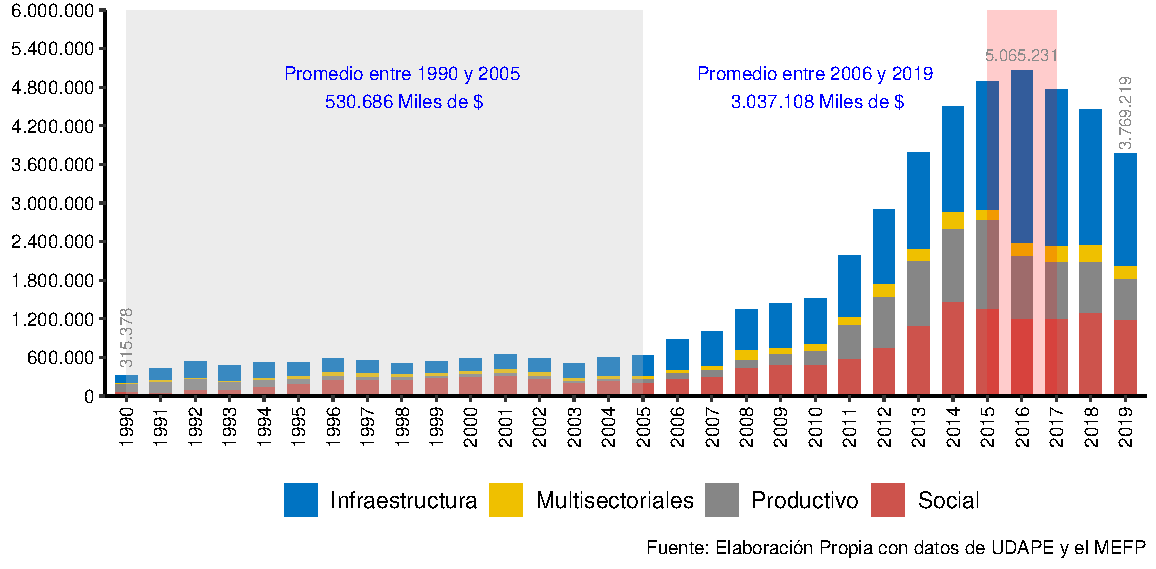
\includegraphics[scale=0.7]{Imagenes/inversion1.pdf}	
\end{figure}


\subsection{Infraestructura}
Un requisito indispensable para mantener el crecimiento de la economía en el largo plazo es contar con la infraestructura que requiere el sector productivo. Esto contribuirá a que
las empresas funcionen con mayor eficiencia y sean más productivas, toda vez que se reflejaría en una disminución de los costos de producción, con un beneficio directo para los consumidores.

Tener carreteras, puertos y ferrocarriles; líneas telefónicas; capacidad de generación, transmisión y distribución de energía eléctrica; una industria petrolera eficiente; presas y canales de irrigación, entre otras obras de infraestructura, es tarea del sector público e indispensable para elevar la competitividad y productividad de las empresas.

Sin embargo, para ello se requiere de una cantidad importante de recursos, que fueron escasos en años pasados dentro del Gobierno Federal, debido a los ajustes presupuestales que éste tuvo que realizar ante la debilidad de sus fuentes de ingresos y los objetivos de tener cuentas equilibradas. Aunque
estos ajustes contribuyeron al fortalecimiento de las finanzas públicas, generaron un rezago importante en materia de
inversión física. 


\section{Modelo}
La notación $AR(p)$ presenta un modelo autorregresivo de orden $p$. El modelo $AR(p)$ se define como:

$${\displaystyle X_{t}=c+\sum _{i=1}^{p}\varphi _{i}X_{t-i}+\varepsilon _{t}\,}$$

donde ${\displaystyle \varphi _{1},\ldots ,\varphi _{p}}{\displaystyle \varphi _{1},\ldots ,\varphi _{p}} $ son los parámetros del modelo, ${\displaystyle c} $es una constante, y ${\displaystyle \varepsilon _{t}}{\displaystyle \varepsilon _{t}}$ es ruido blanco. Esto se puede escribir de manera equivalente usando el operador de retroceso$B$ como

$$ {\displaystyle X_{t}=c+\sum _{i=1}^{p}\varphi _{i}B^{i}X_{t}+\varepsilon _{t}}$$

de manera que, moviendo el término sumatorio hacia el lado izquierdo y el uso de la notación polinómica, tenemos

$${\displaystyle \phi (B)X_{t}=c+\varepsilon _{t}}$$

Un modelo autorregresivo por lo tanto se puede ver como la salida de un todo- polo de impulso respuesta infinito filtro cuya entrada es ruido blanco.

Algunas limitaciones son necesarios en los valores de los parámetros de este modelo con el fin de que el modelo se mantiene estacionario en sentido amplio . Por ejemplo, los procesos $AR(1)$ con el modelo  no son estacionarias. Generalizando, para que un modelo $AR(p)$ sea estacionario en sentido amplio, las raíces del polinomio ${\displaystyle \textstyle z^{p}-\sum _{i=1}^{p}\varphi _{i}z^{p-i}}{\displaystyle \textstyle z^{p}-\sum _{i=1}^{p}\varphi _{i}z^{p-i}}$  debe estar dentro del círculo unitario, es decir, cada raíz ${\displaystyle z_{i}}{\displaystyle z_{i}} $ debe satisface.r

%\newpage


\section{Resultados}
como se observa en el Cuadro \ref{ref:resultados} los resultados 

\begin{table}[!h]
\begin{center}
\caption{\label{ref:resultados}Resultados de las Estimaciones por MCO}
\scalebox{0.85}{
\begin{tabular}{l c c c}
\hline
&&Variable dependiente&\\
& \multicolumn{3}{c}{\textit{Variable dependiente:}} \\
& \multicolumn{3}{c}{\textit{log(Pib\_Real)}} \\
& Model 1 & Model 2 & Model 3 \\
\hline
\hline
(Intercept)          & $12.45^{***}$ & $12.51^{***}$ & $12.32^{***}$ \\
                     & $(0.19)$      & $(0.15)$      & $(0.29)$      \\
log(Infraestructura) & $0.19^{***}$  & $0.18^{***}$  & $0.21^{***}$  \\
                     & $(0.05)$      & $(0.05)$      & $(0.03)$      \\
log(Social)          & $0.12^{**}$   & $0.11^{***}$  & $0.11^{**}$   \\
                     & $(0.03)$      & $(0.03)$      & $(0.03)$      \\
log(Productivo)      & $0.02$        & $0.02$        &               \\
                     & $(0.03)$      & $(0.03)$      &               \\
log(Multisectorial)  & $-0.01$       &               &               \\
                     & $(0.02)$      &               &               \\
\hline

R$^2$                & $0.97$        & $0.97$        & $0.91$        \\
Adj. R$^2$           & $0.97$        & $0.97$        & $0.91$        \\
Num. obs.            & $30$          & $30$          &            \\
rho                  & $$            & $$            & $0.55$        \\
number.interaction   & $$            & $$            & $8.00$        \\
dw.original          & $$            & $$            & $0.67$        \\
p.value.original     & $$            & $$            & $0.00$        \\
dw.transformed       & $$            & $$            & $1.58$        \\
p.value.transformed  & $$            & $$            & $0.04$        \\
nobs                 & $$            & $$            & $30$          \\
\hline
\hline
\multicolumn{4}{l}{\footnotesize{Nota: $^{***}p<0.001$; $^{**}p<0.01$; $^{*}p<0.05$}}
\end{tabular}
%\label{mco}
}
\end{center}
\end{table}  







